\chapter{Polynomials II: Factoring and Rational Functions}


\section{Factoring Polynomials}
We factor a polynomial into two or more polynomials of lower
degree. For example, let's say that you wanted to factor
$5x^3 - 45x$. You would note that you can factor out $5x$ from every term. Thus,
\begin{equation*}
5x^3 - 45x = (5x)(x^2 - 9)
\end{equation*}
You might notice that the second factor looks like the difference of squares, so
\begin{equation*}
5x^3 - 45x = (5x)(x + 3)(x - 3)
\end{equation*}
That is as far as we can factorize this polynomial.\index{factoring polynomials}

Why do we care? The factors make it easy to find the roots of the
polynomial. \index{roots of a polynomial}This polynomial evaluates to zero if and only if at least
one of the factors is zero. Here, we see that
\begin{itemize}
\item The factor $(5x)$ is zero when $x$ is zero.
\item The factor $(x + 3)$ is zero when $x$ is -3.
\item The factor $(x - 3)$ is zero when $x$ is 3.
\end{itemize}
So, looking at the factorization, you can see
that $5x^3 - 45x$ is zero when $x$ is 0, -3, or 3. 

This is a graph of that polynomial with its roots circled:

\begin{figure}[H]
    \centering
    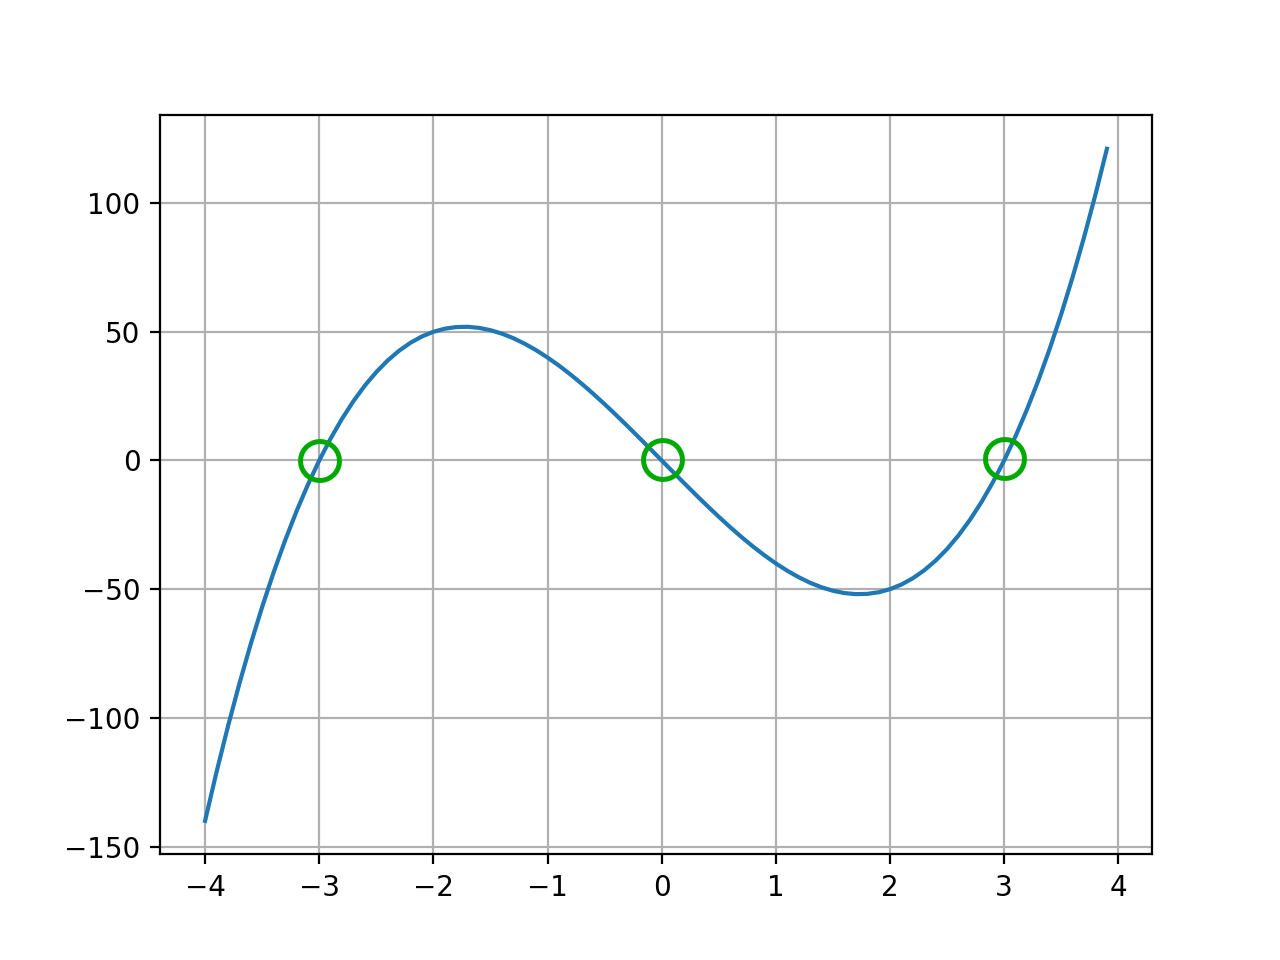
\includegraphics[scale=0.5]{factor4roots.png}
    \caption{Factoring for roots makes it easier to find the roots rather than in expanded form.}
    \label{fig:factor4roots}
\end{figure}


\subsection{How to factor polynomials}\index{greatest common divisor}

The first step when you are trying to factor a polynomial is to find
the greatest common divisor for all the terms, then pull that out. In
this case, the greatest common divisor will also be a monomial. Its
degree is the least of the degrees of the terms, its coefficient will
be the greatest common divisor of the coefficients of the terms.

For example, what can you pull out of this polynomial?
\begin{equation*}
12x^{100} + 30x^{31} + 42x^{17}
\end{equation*}
The greatest common divisor of the coefficients (12, 30, and 42) is 6.  The least of the degrees of terms (100, 31, and 17) is 17.  So, you can pull out $6x^{17}$:
\begin{equation*}
12x^{100} + 30x^{31} + 42x^{17} = (6x^{17})(2x^{83} + 5x^{14} + 7)
\end{equation*}

\begin{Exercise}[title={Factoring out the GCD monomial}, label=gcdmonomial]
Factor out the greatest common divisor monomial from each polynomial.
\begin{enumerate}
\item $18x^3 - 15x$
\item $4x^3 - 12x^2 + 16x$
\item $18x^{50} - 24x^{20} + 30x^{8}$
\end{enumerate}
\end{Exercise}
\begin{Answer}[ref=gcdmonomial]
\begin{enumerate}
\item The GCD of 18 and 15 is 3, and the least degree is 1, so
  $18x^3 - 15x = (3x)(6x^2 - 5)$.
\item The GCD of 4, 12, and 16 is 4, and the least degree is 1, so
  $4x^3 - 12x^2 + 16x = (4x)(x^2 - 3x + 4)$.
\item The GCD of 18, 24, and 30 is 6, and the least degree is 8, so
  $18x^{50} - 24x^{20} + 30x^{8} = (6x^{8})(3x^{42} - 4x^{12} + 5)$.
\end{enumerate}
\end{Answer}
% Items 1-2 adapted from OpenStax, Intermediate Algebra 2e, Ch. 6 Review
% Exercises #343 and #345 (CC BY 4.0):
% https://openstax.org/books/intermediate-algebra-2e/pages/6-review-exercises


So, now you have the product of a monomial and a polynomial. If you
are lucky, the polynomial part looks familiar, like the difference of
squares or a row from Pascal's triangle.

Often, you are trying to \index{factoring!quadratics}factor a quadratic like $x^2 + 5x + 6$ in a pair
of binomials. In this case, the result would be $(x + 3)(x + 2)$. Let's check that:
\begin{equation*}
  (x + 3)(x + 2) = (x)(x) + (3)(x) + (2)(x) + (3)(2) = x^2 + 5x + 6
\end{equation*}
Notice that 3 and 2 multiply to 6 and add to 5. If you were trying to
factor $x^2 + 5x + 6$, you would ask yourself, ``What are two numbers that
when multiplied equal 6 and when added equal 5?'' And you might
guess wrong a couple of times. For example, you might say to yourself,
``Well, 6 times 1 is 6. Maybe those work. But 6 and 1 add 7. So those
don't work.''

Solving these sorts of problems are like solving a Sudoku puzzle. You
try things and realize they are wrong, so you backtrack and try
something else.

The numbers are sometimes negative. For example, $x^2 + 3x - 10$ factors into $(x + 5)(x - 2)$.

\begin{Exercise}[title={Factoring quadratics}, label=factorquadratics]
Factor each quadratic into a pair of binomials.
\begin{enumerate}
\item $x^2 + 14x + 33$
\item $x^2 - 16x + 60$
\item $x^2 + 3x - 54$
\item $x^2 - 3x - 10$
\end{enumerate}
\end{Exercise}
\begin{Answer}[ref=factorquadratics]
\begin{enumerate}
\item 3 and 11 multiply to 33 and add to 14, so
  $x^2 + 14x + 33 = (x + 3)(x + 11)$.
\item $-6$ and $-10$ multiply to 60 and add to $-16$, so
  $x^2 - 16x + 60 = (x - 6)(x - 10)$.
\item 9 and $-6$ multiply to $-54$ and add to 3, so
  $x^2 + 3x - 54 = (x + 9)(x - 6)$.
\item $-5$ and 2 multiply to $-10$ and add to $-3$, so
  $x^2 - 3x - 10 = (x - 5)(x + 2)$.
\end{enumerate}
\end{Answer}
% Adapted from OpenStax, Intermediate Algebra 2e, Ch. 6 Review Exercises
% #355-358 (CC BY 4.0), variables changed to x:
% https://openstax.org/books/intermediate-algebra-2e/pages/6-review-exercises

\index{factoring!checking in Python}\textbf{Computing in Python}

Python can check a factorization for you. Start by writing the
original polynomial and its factored form as two Python functions:

\begin{minted}{python}
def p(x):
    return 5*x**3 - 45*x

def f(x):
    return (5*x)*(x + 3)*(x - 3)
\end{minted}

In Python, \mintinline{python}{**} means ``raised to the power of,'' and
every multiplication needs a \mintinline{python}{*}. You have to write
\mintinline{python}{5*x}, since \mintinline{python}{5x} is an error.

First, confirm the roots we read off the factors:

\begin{minted}{python}
for x in [0, -3, 3, 1]:
    print(x, p(x))
\end{minted}

\begin{minted}{text}
0 0
-3 0
3 0
1 -40
\end{minted}

The values 0, -3, and 3 all give zero, so they are roots. The value 1
gives -40, so it is not a root.

Next, check that \mintinline{python}{p} and \mintinline{python}{f} are
the same polynomial. If the factorization is correct, the two functions
give the same output for every $x$:

\begin{minted}{python}
for x in [0, 1, 2, 3]:
    print(x, p(x), f(x), p(x) == f(x))
\end{minted}

\begin{minted}{text}
0 0 0 True
1 -40 -40 True
2 -50 -50 True
3 0 0 True
\end{minted}

Each line shows $x$, the value of the original, the value of the
factored form, and whether they match. Every line says
\mintinline{python}{True}.

How many values of $x$ do you need to check? Here is a useful fact: if
two polynomials of degree at most $n$ give the same value at $n + 1$ different
values of $x$, they are the same polynomial. Our polynomial has degree
3, so four matching values are enough.

Matching at the roots alone can hide a mistake. Suppose you forgot the 5 when
you pulled out $5x$:

\begin{minted}{python}
def g(x):
    return x*(x + 3)*(x - 3)

for x in [0, -3, 3, 1]:
    print(x, p(x), g(x), p(x) == g(x))
\end{minted}

\begin{minted}{text}
0 0 0 True
-3 0 0 True
3 0 0 True
1 -40 -8 False
\end{minted}

The wrong factorization has the same roots, so it passes at 0, -3, and
3. The value $x = 1$ catches the mistake.

\begin{Exercise}[title={Predict the output}, label={ex:factoring_polynomials-python-1}]
Without running the code, predict what this prints. Which of the two
values of $x$ is a root?
\begin{minted}{python}
def q(x):
    return x**2 + 3*x - 4

print(q(2))
print(q(-4))
\end{minted}
\end{Exercise}
\begin{Answer}[ref={ex:factoring_polynomials-python-1}]
\begin{minted}{text}
6
0
\end{minted}
At $x = 2$: $4 + 6 - 4 = 6$. At $x = -4$: $16 - 12 - 4 = 0$. So $-4$ is
a root and $2$ is not. This matches the factorization
$x^2 + 3x - 4 = (x + 4)(x - 1)$.
\end{Answer}

\begin{Exercise}[title={Spot the sign error}, label={ex:factoring_polynomials-python-2}]
A student claims that $x^2 + 3x - 10 = (x - 5)(x + 2)$ and runs this
check:
\begin{minted}{python}
def a(x):
    return x**2 + 3*x - 10

def b(x):
    return (x - 5)*(x + 2)

for x in [0, 1, 2]:
    print(x, a(x), b(x), a(x) == b(x))
\end{minted}
The output is:
\begin{minted}{text}
0 -10 -10 True
1 -6 -12 False
2 0 -12 False
\end{minted}
The first line says \mintinline{python}{True}. Why is the factorization
still wrong? What is the correct factorization?
\end{Exercise}
\begin{Answer}[ref={ex:factoring_polynomials-python-2}]
At $x = 0$ both sides equal the constant term, $-10$, because $-5$ and
$2$ do multiply to $-10$. A single match proves little here. The polynomial has
degree 2, so all three values must match, and two of them fail. The
numbers $-5$ and $2$ add to $-3$ instead of $3$, so the signs are
swapped. The correct factorization is $(x + 5)(x - 2)$.
\end{Answer}

\begin{Exercise}[title={Spot the bug}, label={ex:factoring_polynomials-python-3}]
A student wants to check that $x^2 + 5x + 6 = (x + 3)(x + 2)$, which we
already know is correct, and writes:
\begin{minted}{python}
def c(x):
    return x^2 + 5*x + 6

def d(x):
    return (x + 3)*(x + 2)

for x in [0, 1, 2]:
    print(x, c(x), d(x), c(x) == d(x))
\end{minted}
The output is:
\begin{minted}{text}
0 8 6 False
1 12 12 True
2 16 20 False
\end{minted}
The factorization is correct, so what went wrong?
\end{Exercise}
\begin{Answer}[ref={ex:factoring_polynomials-python-3}]
In Python, \mintinline{python}{^} does not mean ``to the power of.'' It is
a different operator, so \mintinline{python}{c} computes something
other than $x^2 + 5x + 6$. The fix is to write
\mintinline{python}{x**2}. Notice that the bad version still matches at
$x = 1$ by chance, which is another reason to check several values.
\end{Answer}

\begin{Exercise}[title={Factor, check, and find the roots}, label={ex:factoring_polynomials-python-4}]
Factor $2x^3 - 6x^2 - 8x$ completely. Write the original polynomial and
your factored form as two Python functions, and check that they match
at enough values of $x$. Then use your factors to list the roots, and
confirm that each one gives zero.
\end{Exercise}
\begin{Answer}[ref={ex:factoring_polynomials-python-4}]
Pull out $2x$ to get $(2x)(x^2 - 3x - 4)$. The numbers $-4$ and $1$
multiply to $-4$ and add to $-3$, so
$2x^3 - 6x^2 - 8x = (2x)(x + 1)(x - 4)$.
\begin{minted}{python}
def e(x):
    return 2*x**3 - 6*x**2 - 8*x

def h(x):
    return (2*x)*(x + 1)*(x - 4)

for x in [0, 1, 2, 3]:
    print(x, e(x), h(x), e(x) == h(x))

for r in [0, -1, 4]:
    print(r, e(r))
\end{minted}
The polynomial has degree 3, so four values are enough, and all four
lines say \mintinline{python}{True}. The roots are $0$, $-1$, and $4$,
and each one prints $0$.
\end{Answer}

% Generated without source material; values verified computationally

\index{SymPy}This last part is optional. It uses SymPy, a Python library for
algebra. SymPy is a separate install, so you may need to run
\mintinline{text}{python3 -m pip install sympy} first.

\begin{minted}{python}
from sympy import symbols, factor, expand

x = symbols('x')
print(factor(5*x**3 - 45*x))
print(expand(5*x*(x + 3)*(x - 3)))
\end{minted}

\begin{minted}{text}
5*x*(x - 3)*(x + 3)
5*x**3 - 45*x
\end{minted}

The line \mintinline{python}{x = symbols('x')} makes \mintinline{python}{x}
a \newterm{symbolic variable}\index{symbolic variable}: a letter that
stands for any number, which is how $x$ works in algebra. Earlier in this
section, \mintinline{python}{x} always held one number at a time. Here
it holds no number at all.

The function \mintinline{python}{factor} factors a polynomial, and
\mintinline{python}{expand} multiplies the factors back out. SymPy lists
$(x - 3)$ before $(x + 3)$; the order of the factors does not change
the product.

SymPy also tells you when a polynomial cannot be factored using
integers:

\begin{minted}{python}
print(factor(x**2 + 1))
\end{minted}

\begin{minted}{text}
x**2 + 1
\end{minted}

SymPy returns the polynomial unchanged, so $x^2 + 1$ has no factors
with integer coefficients.

SymPy can factor every polynomial in this chapter in one line, which
means it can also skip the thinking this chapter is teaching. Use it
after you factor by hand, to check your answer.

If you get stuck on a problem, open
\mintinline{text}{factor_hint.py}, type your polynomial
on the line that starts with \mintinline{python}{polynomial =}, and run
the file. It first shows a hint: the polynomial with its greatest common
factor pulled out, found with SymPy's \mintinline{python}{factor_terms}.
Try to finish the problem from there. When you press Enter, the file
shows the full factorization.

\begin{Exercise}[title={Predict what SymPy prints}, label={ex:factoring_polynomials-python-5}]
Without running the code, predict the output.
\begin{minted}{python}
from sympy import symbols, factor

x = symbols('x')
print(factor(x**2 - 9))
\end{minted}
\end{Exercise}
\begin{Answer}[ref={ex:factoring_polynomials-python-5}]
\begin{minted}{text}
(x - 3)*(x + 3)
\end{minted}
The polynomial $x^2 - 9$ is a difference of squares, so it factors into
$(x - 3)(x + 3)$.
\end{Answer}

\begin{Exercise}[title={Factor by hand, then check with SymPy}, label={ex:factoring_polynomials-python-6}]
Factor $3x^2 + 12x - 15$ completely by hand. Then use
\mintinline{python}{expand} to multiply your factors back out, and use
\mintinline{python}{factor} to compare your answer with SymPy's.
\end{Exercise}
\begin{Answer}[ref={ex:factoring_polynomials-python-6}]
Pull out 3 to get $3(x^2 + 4x - 5)$. The numbers $5$ and $-1$ multiply
to $-5$ and add to $4$, so $3x^2 + 12x - 15 = 3(x + 5)(x - 1)$.
\begin{minted}{python}
from sympy import symbols, factor, expand

x = symbols('x')
print(expand(3*(x + 5)*(x - 1)))
print(factor(3*x**2 + 12*x - 15))
\end{minted}
\begin{minted}{text}
3*x**2 + 12*x - 15
3*(x - 1)*(x + 5)
\end{minted}
Expanding gives back the original polynomial, and SymPy's factors match
yours with the binomials in a different order.
\end{Answer}

% SymPy add-on: factor() and expand() usage adapted from GeeksforGeeks, "Python | sympy.factor() method",
% https://www.geeksforgeeks.org/python/python-sympy-factor-method/ ; outputs verified with SymPy


\section{Rational Functions}
We have discussed addition, subtraction, and multiplication of polynomials. What about division?

A quotient of polynomials is called a rational expression.\index{rational!expression} When the polynomials are factored and the stars align, we can \index{rational!simplifying}simplify the rational expression to a single polynomial, just like we might reduce a fraction to lowest terms.

\textbf{Example} 
\begin{equation} \label{eq1}
\begin{split}
\frac{(x + 1)(x + 5)}{x + 5} & = (x + 1) \cdot \frac{x+5}{x+5} \\
& = x + 1 \qquad (x\ne5)
\end{split}
\end{equation}\footnote{It is important to note that we need to restrict $x \ne 5$ since substituting $x=5$ would produce division by zero, making the expression undefined. Canceling the $(x+5)$ factor is only valid when $x \ne 5$, so the simplified form $x+1$ and the original expression are equal everywhere \emph{except} at $x=5$.}

What if the polynomials are not factored? Factor them first.

\textbf{Example} 
\[ \frac{x^2 + 6x + 5}{x + 5} = \frac{(x + 1)(x + 5)}{x + 5} \]
and simplify as in the previous example.

Now, let us consider a rational expression which can be simplified to a single polynomial --- but in the denominator.

\textbf{Example}
\begin{equation} \label{eq1_2}
\begin{split}
\frac{x + 5}{x^2 + 6x + 5} & = \frac{x + 5}{(x + 1)(x + 5)} \\
& = \frac{1}{x+1} \cdot \frac{x+5}{x+5} \\
& = \frac{1}{x+1} \\
\end{split}
\end{equation}

Consider this expression as a function: \( f(x) = \frac{1}{x+1} \). As you might have guessed, this is called a rational function.\index{rational!function} We did not bother looking at the result of the previous example as a function, because we already know that function type: it is a line with slope \( 1 \) and y-intercept \( 1 \). However, this rational function is another animal entirely. Let us examine our first rational function with a familiar concept: the y-intercept. 

\index{y-intercept}y-intercept: \( f(0) =\frac{1}{0 + 1} = \frac{1}{1} = 1 \). The graph contains the point \( (0, 1) \).

Does \( f \) have an \index{x-intercept}x-intercept? That would be an \( x \)-value where \( f(x) = 0 \). But a fraction equals \( 0 \) only when its numerator equals \( 0 \); since the numerator of this expression is always \( 1 \), \( f \) has no x-intercept. 

Knowing the \( y \)-intercept, and that there is no \( x \)-intercept, is a comforting start. But things get weird when we consider a concept that has previously seemed quite simple: domain. Recall that the \index{domain}domain of a function is the set of all values which can be used as inputs. In this case, the domain includes all real numbers, with one exception. The number \( -1 \) is not a valid input because \( f(-1) = \frac{1}{-1+1} = \frac{1}{0} \), which is undefined. So, we say that the domain is all real numbers except \( -1 \). This means the graph contains a point corresponding to every \( x \)-value except \( -1 \).

There is no point at \( x = -1 \), but there is a point at every other \( x \)-value, such as, for example, \( -1.1 \), or \( -0.99999 \). So, what is happening near \( x = -1 \)?

\begin{center}
\begin{tabular}{ |c|c|c|c|c|c|c| } 
 \hline
 x & -1.1 & -1.01 & -1.001 & -0.999 & -0.99 & -0.9 \\ 
 \hline
 f(x) & -10 & -100 & -1000 & 1000 & 100 & 10 \\ 
 \hline
\end{tabular}
\end{center}

The function is going haywire. As we choose \( x \)-values closer and closer to \( -1 \), the resulting function values are larger and larger in magnitude. Also, they are negative on one side, but positive on the other. So, how does a graph go from \( y \)-values of \( -10 \), to \( -100 \), to \( -1000 \), all in a space of less than \( 0.1 \) on the \( x \)-axis? Then, from there, suddenly to big positive numbers on the other side of \( x = -1 \)? All without ever crossing the \( x \)-axis (since there is no \( x \)-intercept)? Let's look at the graph.

\begin{figure}[H]
  \centering
  \begin{tikzpicture}
    \begin{axis}[
      axis lines = middle,
      xlabel = \(x\),
      ylabel = \(f(x)\),
      restrict y to domain = -10:10,
      samples = 100,
    ]
    \addplot [blue, smooth] {1/(x + 1)};
    \end{axis}
  \end{tikzpicture}
  \caption{Graph of \( f(x) = \frac{1}{x+1} \)}
\end{figure}

We can see the \( y \)-intercept we found above. We can also see that the graph has no \( x \)-intercept, as expected. The phenomenon occurring at \( x = -1 \) is called a \index{asymptote}vertical asymptote.\index{vertical!asymptote} One other interesting feature of this graph is how it hugs the \( x \)-axis toward the left and right edges of the window. This makes the line \( y = 0 \) (the \( x \)-axis) a horizontal asymptote for this function.\index{horizontal!asymptote} We can see why this is happening numerically by considering what happens for \( x \)-values far from \( 0 \). In this function, the result is a fraction with a numerator of \( 1 \) and a denominator that is large in size: a fraction that is close to \( 0 \).

\begin{center}
\begin{tabular}{ |c|c|c|c|c|c|c| } 
 \hline
 x & -1000 & -100 & -10 & 10 & 100 & 1000 \\ 
 \hline
 f(x) & -0.001 & -0.01 & -0.1 & 0.1 & 0.01 & 0.001 \\ 
 \hline
\end{tabular}
\end{center}

Let's examine another rational function. Begin by factoring to see if the function can be simplified.
\[ g(x) = \frac{x^2 - 3x + 2}{x^2 - 4x + 3} = \frac{(x - 1)(x - 2)}{(x - 1)(x - 3)} \]
Consider the domain of \( g \) before continuing. Which values of \( x \) are valid inputs? Since substituting \( x = 1 \) or \( x = 3 \) would result in division by \( 0 \), these are not valid inputs. The domain of \( g \) is all real numbers except \( 1 \) and \( 3 \).

Now, for any \( x \)-value except \( 1 \), \( \frac{x-1}{x-1} = 1 \). This means that, for all \( x \)-values but \(1\), we can cancel those factors, leaving \( g(x) = \frac{x-2}{x-3} \). (We will talk more about what is happening at \( x = 1 \) in a moment.)

This function has both \( x \)- and \( y \)-intercepts:
\( y \)-intercept: \( g(0) = \frac{0-2}{0-3} = \frac{2}{3} \). The graph contains the point \( (0, \frac{2}{3}) \).
\( x \)-intercept: \( g(x) = 0 \) where the numerator equals \( 0 \) and the denominator does not equal \( 0 \). Since \( x - 2 = 0 \) when \( x = 2 \), the \( x \)-intercept is \( 2 \) and the graph contains the point \( (2, 0) \).

The graph of \( g \) has a vertical asymptote at any \( x \)-value where substitution would result in dividing a nonzero number by zero. Thus, \( g \) has a vertical asymptote at \( x = 3 \).

Does \( g \) have a horizontal asymptote? Let us see what happens when we substitute \( x \)-values far from \( 0 \).

\begin{center}
\begin{tabular}{ |c|c|c|c|c|c|c| } 
 \hline
 x & -1000 & -100 & -10 & 10 & 100 & 1000 \\ 
 \hline
 g(x) & 0.999 & 0.990 & 0.923 & 1.143 & 1.010 & 1.001 \\ 
 \hline
\end{tabular}
\end{center}

As we move further away from the \( y \)-axis, the \( y \)-values become closer to \( 1 \). The horizontal asymptote describes the end behavior of the function, or what the graph looks like far from the \( y \)-axis.\index{end!behavior} In this case, if we ignore the portion close to the \( y \)-axis, the graph begins to look like the line \( y = 1 \), making this the horizontal asymptote of \( g \). 

So, what is happening at \( x = 1 \)? The value is not in the domain of the function, but there is no vertical asymptote there. That is because substituting any other value for \( x \), even values very close to \( 1 \), into \( \frac{(x - 1)(x - 2)}{(x - 1)(x - 3)} \) gives the exact same number as substituting into \( \frac{x-2}{x-3} \). So, there is a hole in the graph at \( x = 1 \), but nothing strange is happening on either side of \( 1 \).\index{hole} (Depending on the graphing software, the hole may not be visible.)

\begin{figure}[H]
  \centering
  \begin{tikzpicture}
    \begin{axis}[
      axis lines = middle,
      xlabel = \(x\),
      ylabel = \(g(x)\),
      restrict y to domain = -10:10,
      samples = 100,
    ]
    \addplot [red, smooth] {(x - 2)/(x - 3)};
    \end{axis}
  \end{tikzpicture}
  \caption{Graph of \( g(x) = \frac{x^2 - 3x + 2}{x^2 - 4x + 3} \)}
\end{figure}

\begin{Exercise}[title=Rational Functions Practice 1, label=ratfunc1]
  Determine the x- and y-intercepts and horizontal and vertical asymptotes of the rational function:
  \Question{$\frac{2x + 5}{x + 4}$}
  \vspace{40mm}
\end{Exercise}
\begin{Answer}[ref=ratfunc1]
x-intercept: $(-5/2, 0)$; y-intercept: $(0, 5/4)$; horizontal asymptote: $y = 2$; vertical asymptote: $x = -4$
\end{Answer}

\begin{Exercise}[label=ratfunc2]
	[This question was originally presented in the no-calculator section 
	of the 2012 AP Calculus BC exam.] The line $y = 5$ is a horizontal 
	asymptote of which of the following functions? Explain. \\
	A. $y = \frac{\sin{5x}}{x}$\\
	B. $y = 5x$\\
	C. $y = \frac{1}{x-5}$\\
	D. $y = \frac{5x}{1-x}$\\
	E. $y = \frac{20x^2 - x}{1 + 4x^2}$
\end{Exercise}

\begin{Answer}[ref=ratfunc2]
	The correct answer is E. To explain, we examine the behavior of each 
	function as $x \to \infty$. \\
	A. $\lim_{x \to \infty} \frac{\sin{5x}}{x} = \pm \infty \neq 5$\\
	B. $\lim_{x \to \infty} 5x = \infty \neq 5$\\
	C. $\lim_{x \to \infty} \frac{1}{x-5} = 0 \neq 5$ (this function 
	does have a \textit{vertical} asymptote at $x = 5$). \\
	D. $\lim_{x \to \infty} \frac{5x}{1-x} = \frac{5}{-1} = -5 \neq 5$ 
	(this function has a horizontal asymptote at $x = -5$).\\
	E. $\lim_{x \to \infty} \frac{20x^2 - x}{1 + 4x^2} = \frac{20}{4} = 5$. 
\end{Answer}

In those examples, common factors cancel, leaving one polynomial. Of course, there is no guarantee that any two polynomials will have common factors, or even be factorable at all. Now, we consider an example that cannot be simplified. We will focus on just the asymptotes here.
\[ h(x) = \frac{x^2}{x - 1} \]
We see that the \( x \)-value \( 1 \) gives division of a non-zero number by zero, giving a vertical asymptote at \( x = 1 \). How about a horizontal asymptote? We examine values of \( h \) for values of \( x \) far from \( 0 \).

\begin{center}
\begin{tabular}{ |c|c|c|c|c|c|c| } 
 \hline
 x & -1000 & -100 & -10 & 10 & 100 & 1000 \\ 
 \hline
 h(x) & -999 & -99 & -9 & 11 & 101 & 1001 \\ 
 \hline
\end{tabular}
\end{center}

Rather than seeing function values leveling off as in the previous examples, we see function values that grow in size along with \( x \). The function \( h \) has no horizontal asymptote. Let's examine the graph:

\begin{figure}[H]
  \centering
  \begin{tikzpicture}
    \begin{axis}[
      axis lines = middle,
      xlabel = \(x\),
      ylabel = \(h(x)\),
      restrict y to domain = -10:10,
      samples = 100,
    ]
    \addplot [green, smooth] {x^2/(x - 1)};
    \end{axis}
  \end{tikzpicture}
  \caption{Graph of \( h(x) = \frac{x^2}{x - 1} \)}
\end{figure}

This function exhibits a different type of end behavior: that of a line with slope \( 1 \). To see that, cover up the portion of the graph near the \( y \)-axis and focus on the left and right. The rather dull and time-consuming technique of \index{polynomial long division}polynomial long division can be used to rewrite the function as a quotient and a remainder. We encourage you to watch the Khan Academy video on the topic, but for now, let us instead use our knowledge of factoring techniques and a clever little trick.

\begin{equation} \label{eq1_3}
\begin{split}
h(x) & = \frac{x^2}{x - 1} \\
& = \frac{x^2 - 1 + 1}{x - 1} \\ 
& = \frac{x^2 - 1}{x - 1} + \frac{1}{x - 1} \\
& = \frac{(x - 1)(x + 1)}{x - 1} + \frac{1}{x - 1} \\
& = x + 1 + \frac{1}{x - 1}
\end{split}
\end{equation}

We obtain a quotient of \( x + 1 \) and a remainder of \( 1 \). It is the quotient that determines the end behavior of the graph. Why? Substituting \( x \)-values far from zero makes the remainder term very small, since it becomes a fraction with a large denominator but a numerator of only \( 1 \). So for \( x \)-values far from zero, the \( y \)-value is \( x \) plus \( 1 \) plus a very small number (so small that we can justifiably ignore it). This means that far from the \( y \)-axis, the function acts like the quotient: the line \( y = x + 1 \). We call this line an oblique asymptote.\index{oblique!asymptote} See below how the graph of \( h(x) \) hugs that line.

\begin{figure}[H]
  \centering
  \begin{tikzpicture}
    \begin{axis}[
      axis lines = middle,
      xlabel = \(x\),
      ylabel = \(y\),
      restrict y to domain = -10:10,
      samples = 100,
    ]
    \addplot [green, smooth] {x^2/(x - 1)};
    \addplot [black, dashed] {x + 1};    
    \end{axis}
  \end{tikzpicture}
  \caption{Graph of \( h(x) = \frac{x^2}{x - 1} \) and its oblique asymptote \( y = x + 1 \)}
\end{figure}

\begin{Exercise}[title=Rational Functions Practice 2, label=ratfunc2_b]
  Factor and simplify the rational function, then determine any holes and vertical and oblique asymptotes of the rational function.
  \Question{$\frac{x^3 + 2x^2}{x^2 + x}$}
  \vspace{40mm}
\end{Exercise}
\begin{Answer}[ref=ratfunc2_b]Factored form: $\frac{x^2(x + 2)}{x(x + 1)}$; hole: $(0, 0)$; vertical asymptote: $x = -1$; oblique asymptote: $y = x + 1$\end{Answer}

We have seen lines act as end behaviors. Are there other possibilities? Sure! Here is an example with parabolic end behavior. 
\[ k(x) = \frac{x^3}{x - 2} \]
We use our add-subtract trick to reveal the quotient, which describes the end behavior.

\begin{equation} \label{eq1_4}
\begin{split}
h(x) & = \frac{x^3}{x - 2} \\
& = \frac{x^3 - 8 + 8}{x - 2} \\ 
& = \frac{x^3 - 8}{x - 2} + \frac{8}{x - 2} \\
& = \frac{(x - 2)(x^2 + 2x + 4)}{x - 2} + \frac{8}{x - 2} \\
& = x^2 + 2x + 4 + \frac{8}{x - 2}
\end{split}
\end{equation}

The quotient, \( x^2 + 2x + 4 \), should describe the end behavior. We confirm by graphing both \( k \) and the quotient - the \index{parabolic asymptote}parabolic asymptote.

\begin{figure}[H]
  \centering
  \begin{tikzpicture}
    \begin{axis}[
      axis lines = middle,
      xlabel = \(x\),
      ylabel = \(y\),
%      restrict y to domain = -10:10,
      samples = 100,
      xmin = -5, xmax = 7, ymin = -21, ymax = 51,
    ]
    \addplot [purple, smooth] {x^3/(x - 2)};
    \addplot [black, dashed] {x^2 + 2*x + 4};    
    \end{axis}
  \end{tikzpicture}
  \caption{Graph of \( k(x) = \frac{x^3}{x - 2} \) and its parabolic asymptote \( y = x^2 + 2x + 4 \)}
\end{figure}


\section{Partial Fractions}
How can you add fractions with different denominators, like $\frac{1}{x} + 
\frac{2}{x + 3}$? You would need to make the denominators the same; after that, you 
could just add the numerators. You achieve this by multiplying the numerator 
and denominator of each fraction by the denominator of the other fraction:
$$\frac{1}{x} + \frac{2}{x + 3} = \frac{1}{x} \left( \frac{x + 3}{x + 3} 
\right) + \frac{2}{x + 3} \left( \frac{x}{x} \right)$$

Recall that when the numerator and denominator of a fraction are the same, the 
fraction is equal to one. So, we are not changing the \textit{value} of each 
fraction, since we are just multiplying by one. Continuing, we can perform the 
multiplication and see that:
$$\frac{1}{x} + \frac{2}{x + 3} = \frac{x + 3}{x(x + 3)} + \frac{2x}{x(x + 3)}$$
$$= \frac{(x + 3) + 2x}{x(x + 3)} = \frac{3x + 3}{x^2 + 3x} = \frac{3(x + 1)}{x
^2 + 3x}$$

The inverse of this process is called \textbf{partial fraction decomposition} 
(or partial fraction expansion)\index{partial fraction decomposition}. This 
method has applications in many fields, but we will find it most useful as a 
tool to \index{integration}evaluate integrals in a later chapter. 


Let $g(x)$ be a rational function such that 
$$g(x) = \frac{P(x)}{Q(x)}$$
Where $P(x)$ and $Q(x)$ are polynomials. If $g(x)$ is proper (that is, the 
degree of $P$ is less than the degree of $Q(x)$ then we can express $g(x)$ as 
the sum of simpler rational fractions. If $g(x)$ is improper (that is, the 
degree of $P$ is greater than or equal to the degree of $Q$), then we must 
first perform long division to obtain a remainder, $R(x)$, where the degree 
of $R$ is less than the degree of $Q$:
$$g(x) = \frac{P(x)}{Q(x)} = S(x) + \frac{R(x)}{Q(x)}$$

\subsubsection{Improper fractions}\index{improper fraction}
What is $\int \frac{x^3 + x}{x-1}\,dx$. \index{long division}Using long division, we see that:
$$\frac{x^3 + x}{x - 1} = x^2 + x + 2 + \frac{2}{x - 1}$$
(see figure \ref{polylongdiv} for an explanation). Then we can also say that:
$$\frac{x^3 + x}{x-1} = x^2 + x + 2 + \frac{2}{x-1}$$

\begin{figure}[H]
\centering
    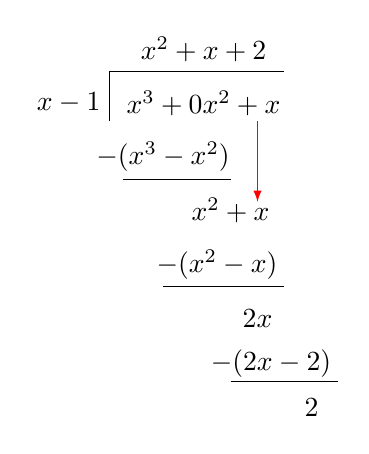
\begin{tikzpicture}
	\begin{axis}[xmin = -1, xmax = 1, axis lines = none, ymin = 0, ymax = 10, 
	clip = false]
            \node[] at (-0.8,8.8) {$x - 1$};
            \draw[black](-0.65, 8.4) -- (-0.65, 9.5);
            \draw[black] (-0.65, 9.5) -- (0, 9.5);
            \node[] at (-0.3, 8.8) {$x^3 + 0x^2 + x$};
            \node[] at (-0.3, 10) {$x^2 + x + 2$};
            \node[] at (-0.45, 7.6) {$-(x^3 - x^2)$};
            \draw[black] (-0.6, 7.1) -- (-0.2, 7.1);
            \node[] at (-0.2, 6.4) {$x^2 + x$};
            \draw[red, -latex](-0.1, 8.4) -- (-0.1, 6.6);
            \node[] at (-0.25, 5.2) {$-(x^2 - x)$};
            \draw[black] (-0.45, 4.7) -- (0, 4.7);
            \node[] at (-0.1, 4) {$2x$};
            \node[] at (-0.05, 3) {$-(2x - 2)$};
            \draw[black] (-0.2, 2.6) -- (0.2, 2.6);
            \node[] at (0.1, 2) {$2$};
        \end{axis}
    \end{tikzpicture}
    \caption{Evaluating $(x^3 + x) \div (x - 1)$ with the long division method}
    \label{polylongdiv}
\end{figure}

When you start with an improper fraction, use long division to reduce it to a 
term plus a proper fraction, then use the methods outlined below to further 
manipulate the proper fraction. 

\begin{Exercise}[label = improper]
Use long division to reduce the following improper rational functions to a 
term plus a proper rational fraction.
\begin{enumerate}
\item $\frac{x^4 + x^3 + 2x^2 + 2x - 3}{x^2 - 3x + 2}$
\item $\frac{2x^3 + 5}{x^3 - 3x^2 + 2x - 4}$
\item $\frac{3x^4 - 2x^3 - x^2 + 1}{x^3 - 3x}$
\end{enumerate}
\end{Exercise}

\begin{Answer}[ref = improper]
\begin{enumerate}
\item $x^2 + 4x + 12 \frac{30x - 27}{x^2 - 3x + 2}$
\item $2 + \frac{6x^2 - 4x + 13}{x^3 - 3x^2 + 2x - 4}$
\item $3x - 2 + \frac{8x^2 - 6x + 1}{x^3 - 3x}$
\end{enumerate}
\end{Answer}

\subsubsection{Proper fractions}\index{proper fraction}
When the order of the numerator is less than or equal to the denominator, 
there are three further possibilities. 

\subsubsection{No repeated linear factors}\index{partial fraction decomposition!distinct linear factors}
In the first case, the denominator, $Q(x)$ is composed of distinct linear 
factors. In this case, we can say that $Q(x) = (a_1x + b_1)(a_2x + b_2) \cdots 
(a_nx + b_n)$, where no factor is repeated (including constant multiples). 
Then, there exists $A, B, C, \cdots$, such that:
$$\frac{P(x)}{Q(x)} = \frac{A}{a_1x+b_1} + \frac{B}{a_2x + b_2} + \cdots$$

Let's see an example of this by decomposing $\frac{4x^2 - 7x - 12}{x (x + 2) (x 
- 3)}$. We start by defining $A$, $B$, and $C$, such that:
$$\frac{4x^2 - 7x - 12}{x (x + 2) (x - 3)} = \frac{A}{x} + \frac{B}{x + 2} + 
\frac{C}{x - 3}$$
Multiplying both sides by $x (x + 2) (x - 3)$ we get:
$$4x^2 - 7x - 12 = A(x + 2)(x - 3) + B(x)(x - 3) + C(x)(x + 2)$$
We have 3 unknowns and only one equation! Don't worry --- remember this equation 
is true for all $x$, so we can choose a convenient value of $x$ to isolate 
each unknown in turn. Starting, let $x = 0$. Then:
$$4(0)^2 - 7(0) - 12 = A(0 + 2)(0 - 3) + B(0)(x - 3) + C(0)(x + 2)$$
$$-12 = A(2)(-3) + 0 + 0$$
Notice that the $B$ and $C$ disappear, and we can solve for $A$:
$$A = \frac{-12}{-6} = 2$$
We can solve for $B$ by setting $x = -2$ and for $C$ by setting $x = 3$ 
(notice, we've used all three zeroes of the denominator polynomial):
$$4(-2)^2 - 7(-2) - 12 = A(-2 + 2)(-2 - 3) + B(-2)(-2 - 3) + C(-2)(-2 + 2)$$
$$4(4) + 14 - 12 = 0 + B(-2)(-5) + 0$$
$$16 + 2 = 10B$$
$$B = \frac{9}{5}$$
and
$$4(3)^2 - 7(3) - 12 = A(3 + 2)(3 - 3) + B(3)(3 - 3) + C(3)(3 + 2)$$
$$4(9) - 21 - 12 = 0 + 0 + C(3)(5)$$
$$36 - 33 = 15C$$
$$C = \frac{1}{5}$$
We can then decompose our original fraction:
$$\frac{4x^2 - 7x - 12}{x (x + 2) (x - 3)} = \frac{2}{x} + \frac{9}{5(x + 2)} 
+ \frac{1}{5(x - 3)}$$
You can check your answer by cross-multiplying and adding. You should get the 
same rational function back. 

\subsubsection{Repeated linear factors}\index{partial fraction decomposition!repeated linear factors}
The second case is if $Q(x)$ has repeated factors (such as $x^2 + 8x + 16 = (x 
+ 4)^2$). Suppose the first linear factor, $(a_1x + b_1)$ is repeated $r$ 
times (that is, $Q(x)$ contains the factor $(a_1x + b_1)^r$). Then, instead of 
$\frac{A}{a_1x + b_1}$, we should write:
$$\frac{A_1}{a_1x + b_1} + \frac{A_2}{(a_1x + b_1)^2} + \cdots + \frac{A_r}{(
a_1x + b_1)^r}$$
Let's look at a concrete example to see how this works:

\textbf{Example}: Decompose $\frac{x^2 + x + 1}{(x + 1)^2 (x + 2)}$

\textbf{Solution}: We start by defining:
$$\frac{x^2 + x + 1}{(x + 1)^2 (x + 2)} = \frac{A}{x + 1} + \frac{B}{(x + 1)^
2} + \frac{C}{x + 2}$$
Multiplying both sides by $(x + 1)^2 (x + 2)$:
$$x^2 + x + 1 = A(x + 1)(x + 2) + B(x + 2) + C(x + 1)^2$$
Since there are only 2 roots to $(x + 1)^2 (x + 2)$, we will use another 
method called ''equating the coefficients" to find $A$, $B$, and $C$. We start 
by expanding the right side of the equation:
$$x^2 + x + 1 = A(x^2 + 3x + 2) + B(x + 2) + C(x^2 + 2x + 1)$$
Distributing and combining, we find that:
$$x^2 + x + 1 = Ax^2 + 3Ax + 2A + Bx + 2B + Cx^2 + 2Cx + C$$
$$x^2 + x + 1 = (A + C)x^2 + (3A + B + 2C)x + (2A + 2B + C)$$
For this equation to be true, we know that:
$$A + C = 1$$
$$3A + B + 2C = 1$$
$$2A + 2B + C = 1$$
(That is, the coefficient for $x^2$ on the left, 1, must be equal to the 
coefficient for $x^2$ on the right, (A + C), and so on.) We now have a system 
of 3 equations and 3 unknowns. When you solve for each, you should find that:
$$A = -2$$
$$B = 1$$
$$C = 3$$
Therefore, 
$$\frac{x^2 + x + 1}{(x + 1)^2 (x + 2)} = \frac{-2}{x + 1} + \frac{1}{(x + 1)^
2} + \frac{3}{x + 2}$$

\subsubsection{Irreducible quadratic factors}\index{partial fraction decomposition!irreducible quadratic factors}
Sometimes, we cannot express a polynomial as the product of two linear 
statements (that is, terms in the form $ax + b$). Take $x^2 + 1$, which 
cannot be expressed as the product of real, linear terms. What do you do 
if something like $x^2 + 1$ is in the denominator? In this case, when we write an 
expression for $\frac{P(x)}{Q(x)}$, we include a term in the form:
$$\frac{Ax + B}{ax^2 + bx + c}$$
For example, we can write:
$$\frac{x}{(x - 2)(x^2 + 1)(x^2 + 4)} = \frac{A}{x - 2} + \frac{Bx + C}{x^2 + 1} 
+ \frac{Dx + E}{x^2 + 4}$$

\textbf{Example}: Decompose $\frac{2x^2 - x + 4}{x^3 + 4x}$

\textbf{Solution}: We begin by factoring the denominator:
$$x^3 + 4x = x(x^2 + 4)$$
Which cannot be factored further. Therefore, we define:
$$\frac{2x^2 - x + 4}{x(x^2 + 4)} = \frac{A}{x} + \frac{Bx + C}{x^2 + 4}$$
$$2x^2 - x + 4 = A(x^2 + 4) + (Bx + C)x$$
$$2x^2 - x + 4 = Ax^2 + 4A + Bx^2 + Cx$$
Which implies that:
$$2 = A + B$$
$$C = -1$$
$$4A = 4$$
Therefore, $A = 1$, $B = 1$, and $C = -1$ and we can say that:
$$\frac{2x^2 - x + 4}{x^3 + 4x} = \frac{1}{x} + \frac{x - 1}{x^2 + 4}$$

\subsubsection{Repeated irreducible quadratic factors}
Lastly, the denominator might contain repeated irreducible quadratic factors. 
Similar to repeated linear factors, when setting up your partial fractions, 
instead of only writing 
$$\frac{A}{ax^2 + bx + c}$$
For a quadratic factor that is repeated $r$ times, your equation should include:
$$\frac{A_1}{ax^2 + bx + c} + \frac{A_2}{(ax^2 + bx + c)^2} + \cdots + 
\frac{A_r}{(ax^2 + bx + c)^r}$$

\begin{Exercise}[label = proper]
Decompose the following proper fractions
\begin{enumerate}
\item $\frac{x - 4}{x^2 + 5x - 6}$
\item $\frac{x^2 + x + 1}{(x^2 + 1)^2}$
\item $\frac{x^2 + x + 1}{(x + 1)^2 (x + 2)}$
\end{enumerate}
\end{Exercise}

\begin{Answer}[ref = proper]
\begin{enumerate}
\item $\frac{10}{7(x + 6)} + \frac{-3}{7(x - 1)}$
\item $\frac{1}{x^2 + 1} + \frac{x}{(x^2 + 1)^2}$
\item $\frac{-2}{x + 1} + \frac{1}{(x + 1)^2} + \frac{3}{x + 2}$
\end{enumerate}
\end{Answer}
